\subsection{Examples}

\begin{concept}{Branch Types Overview}\\
Three main classifications of branches:

\textbf{By Condition:}
\begin{itemize}
  \item \textbf{Unconditional}: Branch always
  \item \textbf{Conditional}: Branch only if condition is met
\end{itemize}

\textbf{By Target Address:}
\begin{itemize}
  \item \textbf{Relative}: Target address relative to PC
  \item \textbf{Absolute}: Complete target address
\end{itemize}

\textbf{By Address Hand-over:}
\begin{itemize}
  \item \textbf{Direct}: Target address part of instruction
  \item \textbf{Indirect}: Target address in register
\end{itemize}

%\includegraphics[width=\linewidth]{images/branch_overview.png}
\end{concept}

\begin{example2}{Unconditional Branch Flow}\\
Example of branching sequence and jump table:
\begin{lstlisting}[language=armasm, style=basesmol]
Label1  LDR     R0, =Label5
Label2  BX      R0
Jumptable
        DCD     Case0
        DCD     Case1
        DCD     Case2
        DCD     Case3
Label5  LDR     R0, =Label6
        B       Label2
Label6  LDR     R2, =Jumptable
        ADDS    R2, R2, #4
Label4  LDR     R2, [R2]
        BX      R2
Case0   B       Case0           ; Infinite loop
Case1   B       Label1
Case2   B       Label1
Case3   B       Case0
\end{lstlisting}
\end{example2}

\begin{KR}{Branch Pattern Recognition}\\
Common branch patterns and their uses:

1. Basic branching:
\begin{lstlisting}[language=armasm, style=basesmol]
    ; Simple jump
    B       target          ; Unconditional
    BEQ     target          ; Branch if equal
    BNE     target          ; Branch if not equal
    
    ; Conditional execution
    CMP     R0, #value
    BCC     target          ; Branch if carry clear
    BGT     target          ; Branch if greater than
\end{lstlisting}

2. Jump tables:
\begin{lstlisting}[language=armasm, style=basesmol]
    ; Load table base
    LDR     R0, =jumptable
    ; Calculate offset
    LSLS    R1, R1, #2      ; Multiply index by 4
    ADDS    R0, R0, R1      ; Add to base
    ; Jump to handler
    LDR     R0, [R0]        ; Load address
    BX      R0              ; Branch to handler
\end{lstlisting}

3. Infinite loops:
\begin{lstlisting}[language=armasm, style=basesmol]
endless B       endless      ; Simple infinite loop

loop    ; Do something
        B       loop        ; Loop forever
\end{lstlisting}
\end{KR}

\begin{example2}{Conditional Branches with Flag Testing}\\
Example tracking non-taken branches:
\begin{lstlisting}[language=armasm, style=basesmol]
    MOVS    R0, #0          ; Clear mask
    
    ; Test carry flag
    ADDS    R1, R1, #5
    BCS     taken
    ADDS    R0, R0, #0x01   ; Mark if not taken
taken

    ; Test equality
    ANDS    R1, R1, R5
    BEQ     equal
    ADDS    R0, R0, #0x02   ; Mark if not taken
equal

    ; Test overflow
    SUBS    R2, R2, R5
    BVS     overflow
    ADDS    R0, R0, #0x04   ; Mark if not taken
overflow
\end{lstlisting}

Result in R0 shows which branches were not taken.
\end{example2}

\begin{example2}{Comparison Instructions}\\
Using CMP and TST instructions:
\begin{lstlisting}[language=armasm, style=basesmol]
    ; Signed comparisons
    LDR     R1, =0xFFFFFFFF
    CMP     R1, #1          ; Compare with immediate
    BLT     is_less         ; Branch if less than
    
    ; Unsigned comparisons
    CMP     R1, #1
    BLO     is_below        ; Branch if lower
    
    ; Bit testing
    LDR     R5, =0x0040FFFF
    TST     R3, R5          ; Test bits
    BNE     bits_set        ; Branch if any bit set
    BEQ     bits_clear      ; Branch if all bits clear
\end{lstlisting}
\end{example2}

\begin{KR}{Flow Control Implementation}\\
Guidelines for implementing control structures:

1. If-Then-Else:
\begin{lstlisting}[language=armasm, style=basesmol]
    ; if (condition) {
    ;     then-part
    ; } else {
    ;     else-part
    ; }
    CMP     R0, #value      ; Test condition
    BNE     else_part       ; Branch if false
then_part
    ; Then code
    B       endif           ; Skip else
else_part
    ; Else code
endif
\end{lstlisting}

2. Switch-Case:
\begin{lstlisting}[language=armasm, style=basesmol]
    ; switch(value) {
    ;    case 0: ... break;
    ;    case 1: ... break;
    ; }
    LDR     R0, =jumptable
    LSLS    R1, R1, #2      ; Index * 4
    ADD     R0, R1          ; Add to base
    LDR     R0, [R0]        ; Get handler
    BX      R0              ; Jump to handler

jumptable
    DCD     case0
    DCD     case1
\end{lstlisting}

3. Loops:
\begin{lstlisting}[language=armasm, style=basesmol]
    ; while (condition) {
    ;     body
    ; }
    B       test            ; Jump to test
loop
    ; Loop body
test
    CMP     R0, #value      ; Test condition
    BLT     loop           ; Continue if true
\end{lstlisting}
\end{KR}

\begin{remark}
Important considerations:
\begin{itemize}
  \item Consider branch range limitations
  \item Be aware of condition flag changes
  \item Handle corner cases in comparisons
  \item Plan for proper loop termination
  \item Document complex branching logic
\end{itemize}
\end{remark}

\section*{CT1 Exercises for Branching Instructions}
\section*{Content}
CT1 Exercises for Branching Instructions ..... 1\\
Exercise 1 - Unconditional Branches ..... 2\\
Exercise 2 - Conditional Branches ..... 3\\
Exercise 3 - Comparison Instructions ..... 4\\
Solutions ..... 5\\
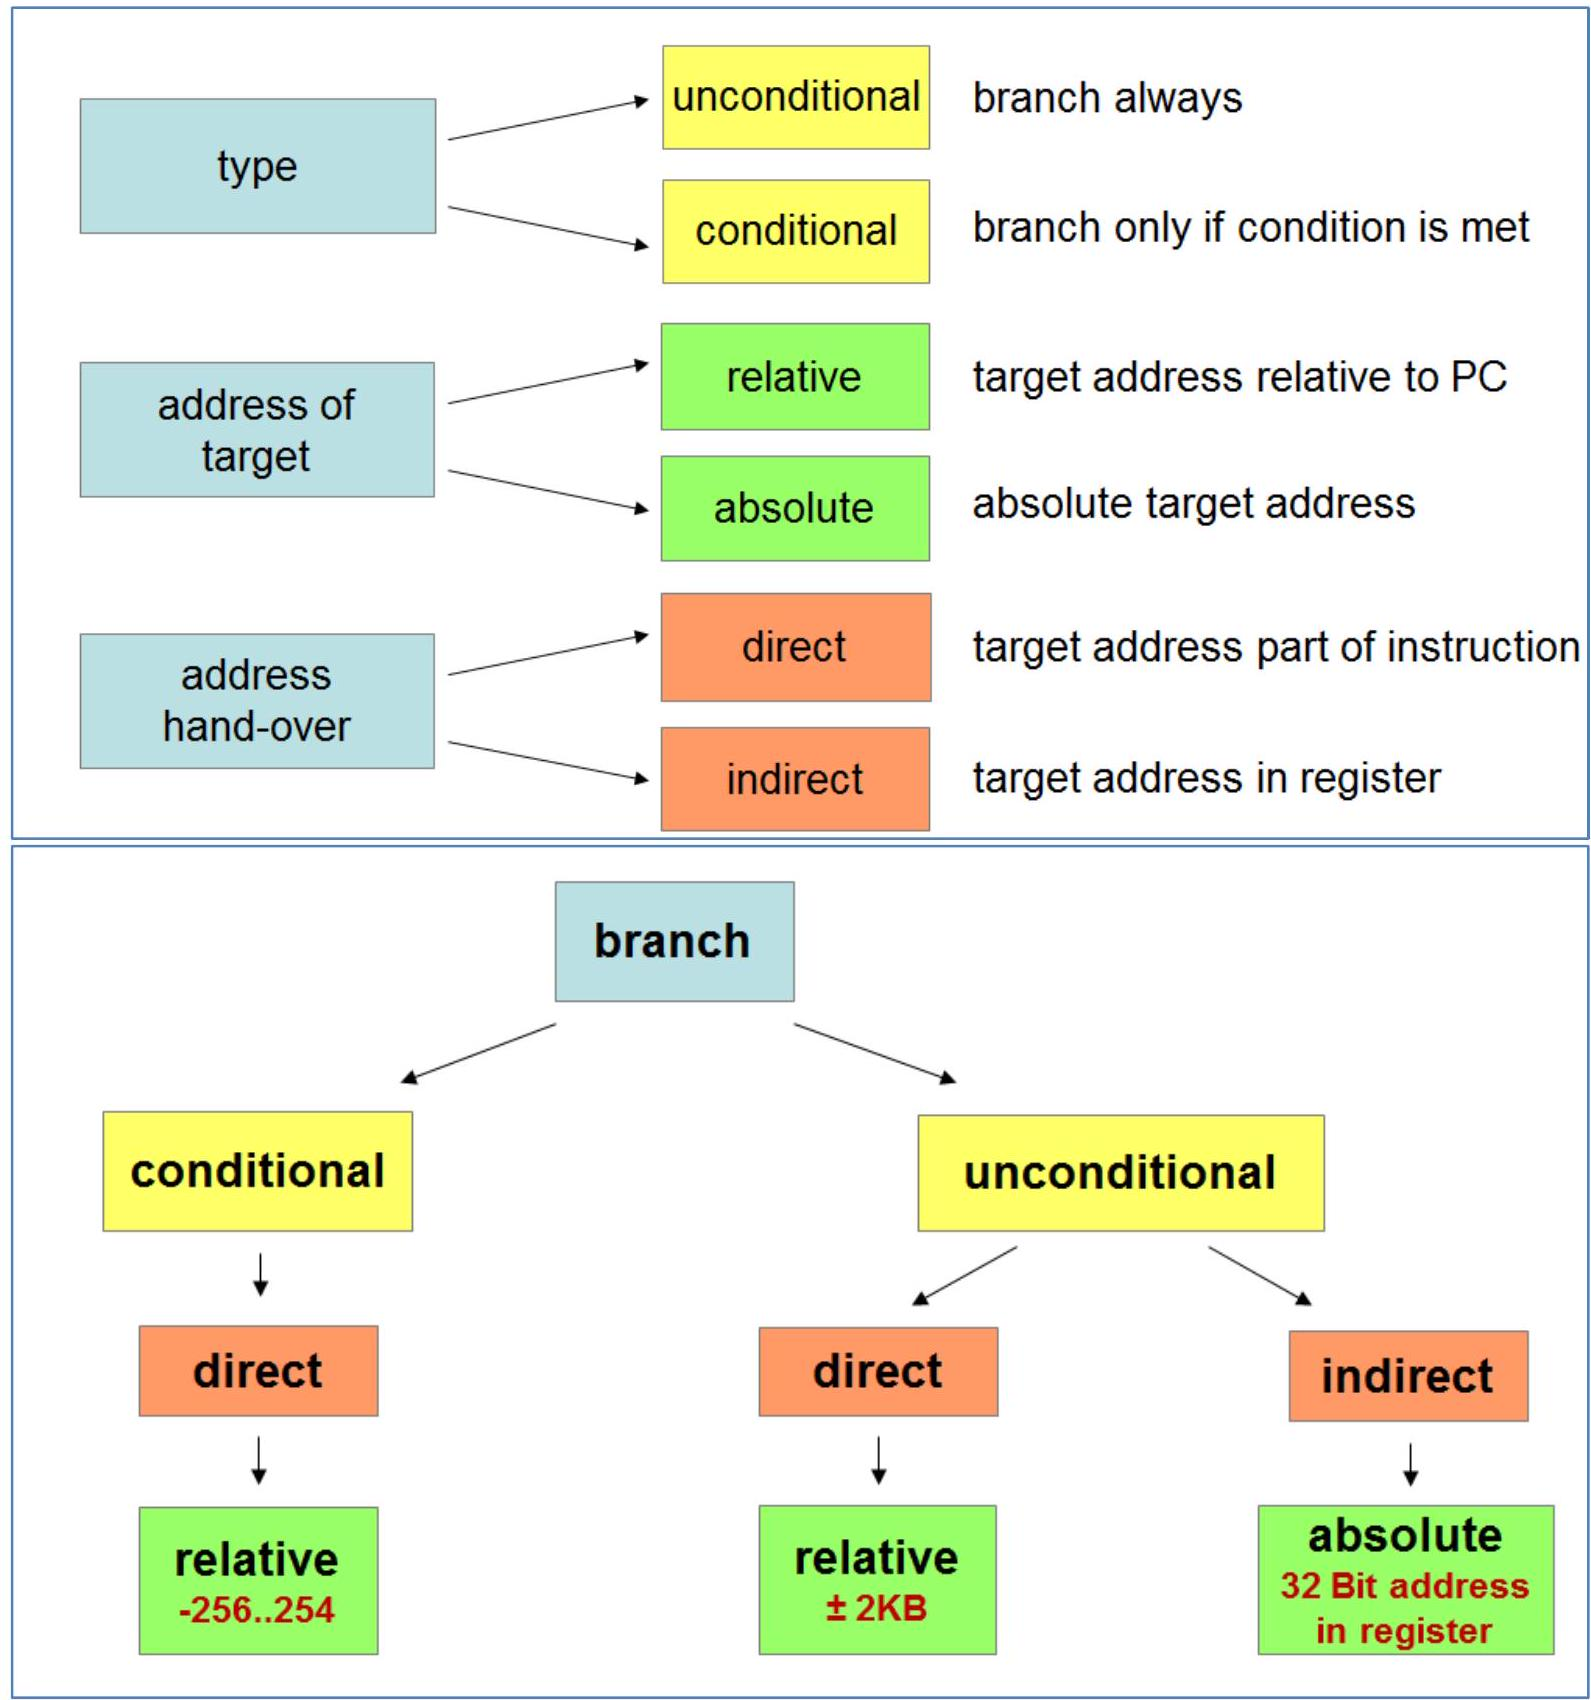
\includegraphics[width=\linewidth]{images/2025_01_02_9902c2d2685de638ef73g-1}

\section*{Exercise 1 - Unconditional Branches}
The execution starts at line 10.

\begin{enumerate}
  \item List the sequence of branch instructions that end in an infinite loop.
\end{enumerate}

Do this by stating the branches in tabular form: from - to.\\
E.g. the first branch is $\underline{\mathbf{1 1 - 1 6}}$ (branch unconditionally from line 11 to line 16).\\
2) At which line does the execution sequence finally loop forever?

\begin{center}
\begin{tabular}{|l|lll|}
\hline
10 & Label1 & LDR & R0, =Label5 \\
11 & Label2 & BX & R0 \\
12 & Jumptable & DCD & Case0 \\
13 &  & DCD & Case1 \\
14 &  & DCD & Case2 \\
15 &  & DCD & Case3 \\
16 & Label5 & LDR & R0, =Label6 \\
17 &  & B & Label2 \\
18 & Label6 & LDR & R2, =Jumptable \\
19 &  & ADDS R2, R2, \#4 &  \\
20 & Label4 & LDR R2, [R2] &  \\
21 &  & BX & R2 \\
22 & Case0 & B & Case0 \\
23 & Case1 & LDR & R2, =Jumptable \\
24 &  & MOVS R1, \#3 &  \\
25 &  & LSLS R1, R1, \#2 &  \\
26 &  & ADDS R2, R2, R1 &  \\
27 &  & B & Label4 \\
28 & Case2 & B & Label1 \\
29 & Case3 & B & Case0 \\
\hline
\end{tabular}
\end{center}

Your solution (the number of cells below is no hint)\\
1)

\begin{center}
\begin{tabular}{|l|l|l|l|l|l|l|l|}
\hline
$11-16$ &  &  &  &  &  &  &  \\
\hline
\end{tabular}
\end{center}

2.

\section*{Exercise 2 - Conditional Branches}
The execution starts at line 10.

\begin{enumerate}
  \item List which branch instructions jump to the given label.
\end{enumerate}

Do this by stating the branches in tabular form: from - to.\\
2) What is the final value in $R 0$ as hexadecimal value?\\
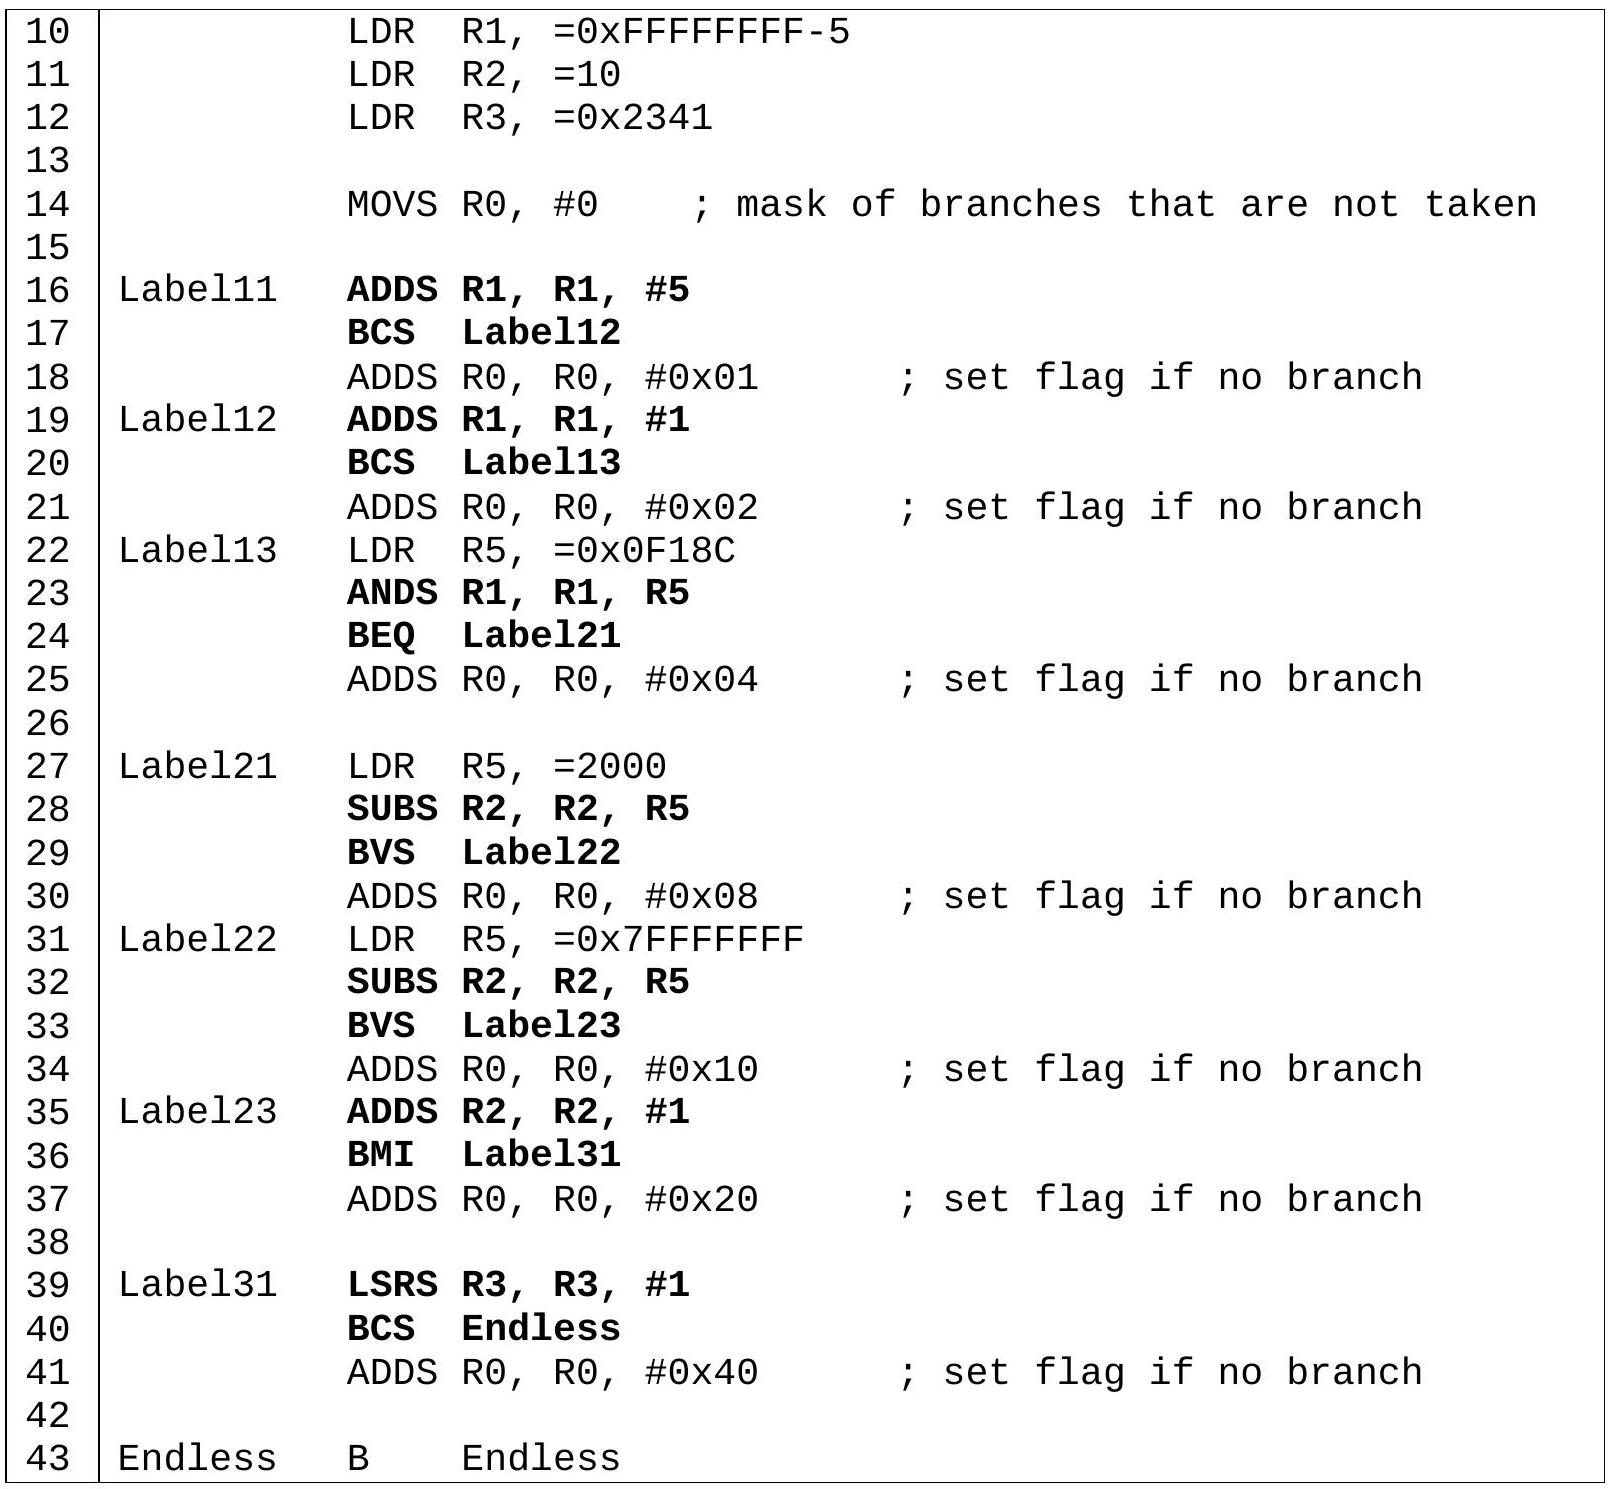
\includegraphics[width=\linewidth]{images/2025_01_02_9902c2d2685de638ef73g-3}

Your solution (the number of cells below is no hint)

\begin{enumerate}
  \item $\square$
  \item $\quad R 0=0 x$. $\qquad$
\end{enumerate}

\section*{Exercise 3 - Comparison Instructions}
The execution starts at line 10.

\begin{enumerate}
  \item List which branch instructions jump to the given label.
\end{enumerate}

Do this by stating the branches in tabular form: from - to.\\
2) What is the final value in $R 0$ as hexadecimal value?\\
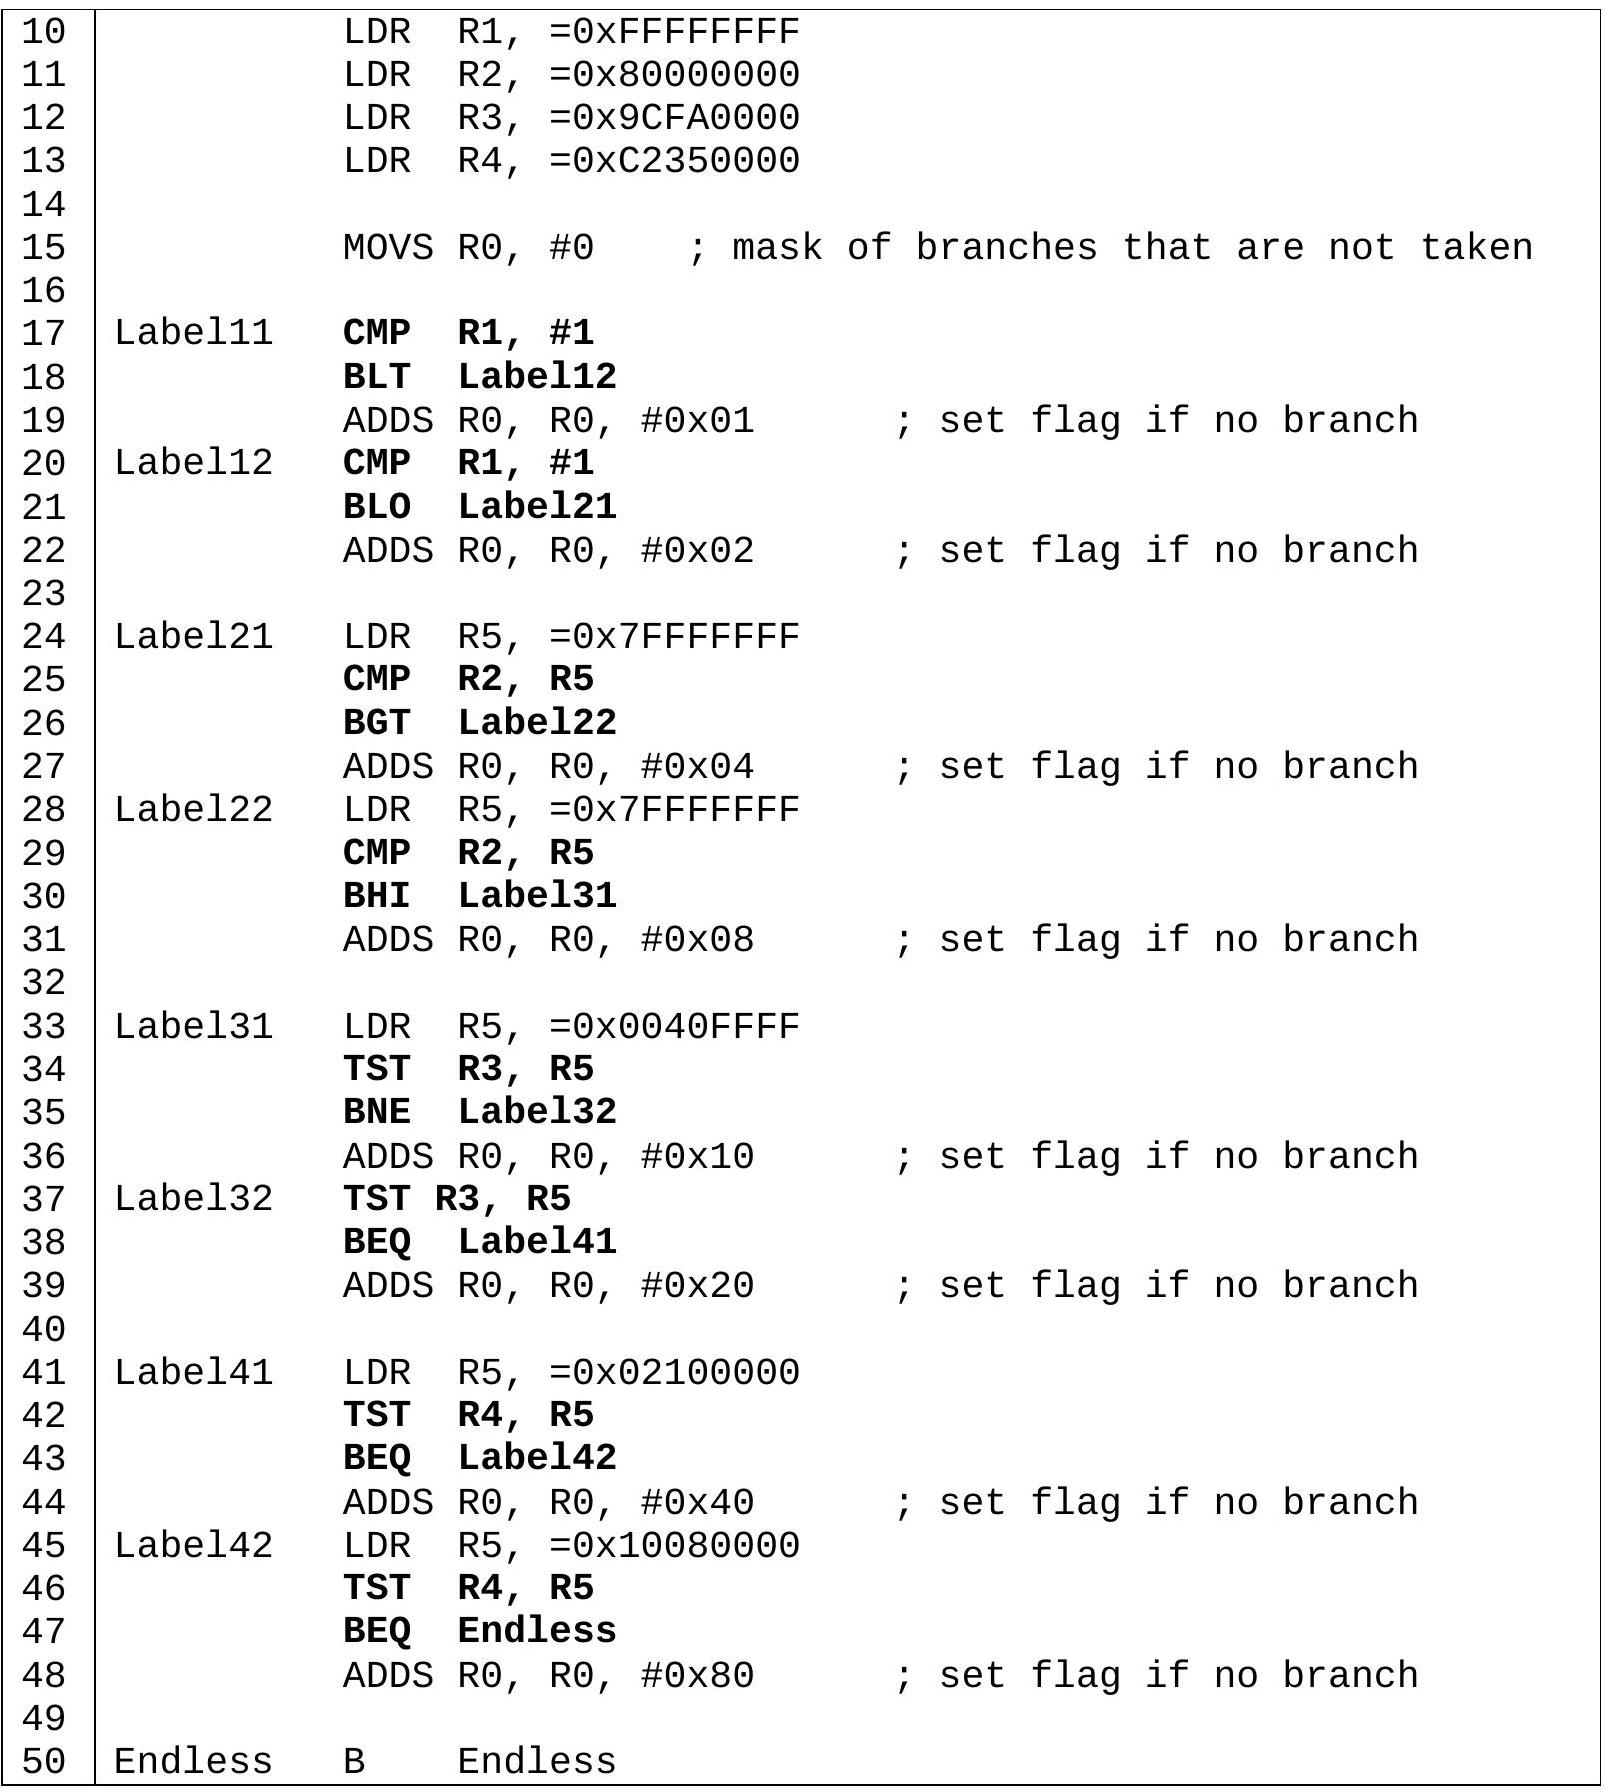
\includegraphics[width=\linewidth]{images/2025_01_02_9902c2d2685de638ef73g-4}

Your solution (the number of cells below is no hint)

\begin{enumerate}
  \item $\square$
  \item $\quad R O=0 x$. $\qquad$
\end{enumerate}

\section*{Solutions}
\section*{Exercise 1:}
\begin{enumerate}
  \item $10-16,17-11,11-18,21-23,27-20,21-29,29-22,22-22 \ldots$
  \item Loops at line 22
\end{enumerate}

\section*{Exercise 2:}
\begin{enumerate}
  \item $20-22,24-27,33-35,40-43$
  \item $0 \times 29$ (binary 0010 '1001)
\end{enumerate}

\section*{Exercise 3:}
\begin{enumerate}
  \item $18-20,30-33,35-37,47-50$
  \item $0 \times 66$ (binary 0110 '0110)
\end{enumerate}

\subsection{Examples}

\begin{concept}{Control Structure Types}\\
Three fundamental types of control structures:

\textbf{1. Sequence}:
\begin{itemize}
  \item Linear execution of instructions
  \item No branching or decisions
  \item Operations performed in order
\end{itemize}

\textbf{2. Selection}:
\begin{itemize}
  \item Conditional execution (if-then-else)
  \item Branch based on condition
  \item Different paths based on test
\end{itemize}

\textbf{3. Iteration}:
\begin{itemize}
  \item Repeated execution (loops)
  \item Condition-controlled repetition
  \item Fixed number of repetitions
\end{itemize}

%\includegraphics[width=\linewidth]{images/control_structures_overview.png}
\end{concept}

\begin{example2}{Selection Structures}\\
If-Then-Else with unsigned 8-bit variables:

\begin{lstlisting}[language=C, style=basesmol]
// C code
uint8_t nrX = ...;
uint8_t nrY = ...;
if (nrX > nrY) {
    nrX = nrY;
} else {
    nrY = nrX;
}
\end{lstlisting}

Assembly implementation:
\begin{lstlisting}[language=armasm, style=basesmol]
    AREA    progCode, CODE, READONLY
    THUMB
main
    PROC
    EXPORT  main
    
    LDR     R6, =nrX      ; R6 = address of nrX
    LDRB    R0, [R6]      ; R0 = byte stored at nrX
    LDR     R7, =nrY      ; R7 = address of nrY
    LDRB    R1, [R7]      ; R1 = byte stored at nrY
    CMP     R0, R1
    BLS     else          ; *unsigned* comparison
    STRB    R1, [R6]      ; store nrY value at nrX
    B       endif
else
    STRB    R0, [R7]      ; store nrX value at nrY
endif
    ENDP
\end{lstlisting}
\end{example2}

\begin{KR}{Selection Implementation}\\
Guidelines for implementing if-then-else structures:

1. Single condition:
\begin{lstlisting}[language=armasm, style=basesmol]
    ; if (condition) {
    ;     then-part
    ; } else {
    ;     else-part
    ; }
    
    ; Test condition
    CMP     Rx, Ry            ; Compare values
    B<cc>   else_label        ; Branch if condition false
    
    ; Then part
    <then instructions>
    B       endif_label       ; Skip else part
    
else_label
    ; Else part
    <else instructions>
    
endif_label
    ; Continue execution
\end{lstlisting}

2. Multiple conditions (AND):
\begin{lstlisting}[language=armasm, style=basesmol]
    ; if (condA && condB) {
    ;     then-part
    ; } else {
    ;     else-part
    ; }
    
    ; Test first condition
    CMP     Rx, #valA
    B<cc>   else_label        ; Branch if first fails
    
    ; Test second condition
    CMP     Ry, #valB
    B<cc>   else_label        ; Branch if second fails
    
    ; Then part
    <then instructions>
    B       endif_label
    
else_label
    ; Else part
    <else instructions>
    
endif_label
\end{lstlisting}

3. Multiple conditions (OR):
\begin{lstlisting}[language=armasm, style=basesmol]
    ; if (condA || condB) {
    ;     then-part
    ; } else {
    ;     else-part
    ; }
    
    ; Test first condition
    CMP     Rx, #valA
    B<cc>   test_second       ; Try second if first fails
    B       then_label        ; First succeeded
    
test_second
    CMP     Ry, #valB
    B<cc>   else_label        ; Branch if both fail
    
then_label
    ; Then part
    <then instructions>
    B       endif_label
    
else_label
    ; Else part
    <else instructions>
    
endif_label
\end{lstlisting}
\end{KR}

\begin{example2}{For-Loop Implementation}\\
Example for-loop in C and assembly:

\begin{lstlisting}[language=C, style=basesmol]
// C code with volatile variables
volatile int32_t i = 0;
volatile int32_t count = 0;
for(i = 0; i < 10; i++) {
    count++;
}
\end{lstlisting}

Assembly implementation:
\begin{lstlisting}[language=armasm, style=basesmol]
    AREA    progCode, CODE, READONLY
    THUMB
main
    PROC
    EXPORT  main
    
    LDR     R6, =i          ; R6 = address of i
    LDR     R0, [R6]        ; R0 = value at i
    LDR     R7, =count      ; R7 = address of count
    LDR     R1, [R7]        ; R1 = value at count
    B       cond
    
loop
    ADDS    R0, R0, #1      ; Increment i
    ADDS    R1, R1, #1      ; Increment count
cond
    CMP     R0, #10
    BLT     loop            ; Branch if i < 10
    
    STR     R0, [R6]        ; Store final i
    STR     R1, [R7]        ; Store final count
    ENDP
\end{lstlisting}

Compiler-optimized version:
\begin{lstlisting}[language=armasm, style=basesmol]
    LDR     r1, [pc, #20]   ; Load address
    MOVS    r0, #0          ; Initialize counter
    STR     r0, [r1, #0]    ; Store i
    LDR     r2, [r1, #4]    ; Load count
    
increment
    ADDS    r0, r0, #1      ; i++
    ADDS    r2, r2, #1      ; count++
    CMP     r0, #10         ; Check condition
    BLT     increment       ; Loop if i < 10
    STM     r1!, {r0, r2}   ; Store final values
\end{lstlisting}
\end{example2}

\begin{example2}{String Processing Loop}\\
Converting string to uppercase:
\begin{lstlisting}[language=armasm, style=basesmol]
    AREA    progCode, CODE, READONLY
    THUMB
main
    PROC
    EXPORT  main
    LDR     R0, =srcstr     ; Source string
    LDR     R1, =outstr     ; Output string
    MOVS    R2, #0          ; Initialize index
    
cond
    LDRB    R3, [R0, R2]    ; Load character
    CMP     R3, #0          ; Check for end
    BEQ     endloop         ; Exit if done
    CMP     R3, #60         ; Check if < 'a'
    BLO     store           ; Skip if not lowercase
    CMP     R3, #90         ; Check if > 'z'
    BHI     store           ; Skip if not lowercase
    ADDS    R3, R3, #32     ; Convert to uppercase
    
store
    STRB    R3, [R1, R2]    ; Store character
    ADDS    R2, R2, #1      ; Next character
    B       cond            ; Continue loop
    
endloop
    STRB    R3, [R1, R2]    ; Store terminator
    ENDP
    
srcstr  DCB     "This IS mY TestStriNG", 0
    AREA    progData, DATA, READWRITE
outstr  SPACE   50
\end{lstlisting}

Result: "THIS IS MY TESTSTRING"
\end{example2}

\begin{KR}{String Processing Patterns}\\
Common patterns for string manipulation:

1. String traversal:
\begin{lstlisting}[language=armasm, style=basesmol]
    MOVS    R2, #0          ; Index
loop
    LDRB    R3, [R0, R2]    ; Load char
    CMP     R3, #0          ; Check end
    BEQ     done            ; Exit if terminator
    ; Process character
    ADDS    R2, R2, #1      ; Next char
    B       loop
\end{lstlisting}

2. Character transformation:
\begin{lstlisting}[language=armasm, style=basesmol]
    ; Check character range
    CMP     R3, #lower_bound
    BLO     skip            ; Below range
    CMP     R3, #upper_bound
    BHI     skip            ; Above range
    
    ; Transform character
    ADDS    R3, #offset     ; Apply offset
    
skip
    STRB    R3, [R1, R2]    ; Store result
\end{lstlisting}

3. String copy:
\begin{lstlisting}[language=armasm, style=basesmol]
    MOVS    R2, #0          ; Index
copy_loop
    LDRB    R3, [R0, R2]    ; Load source
    STRB    R3, [R1, R2]    ; Store to dest
    ADDS    R2, R2, #1      ; Next char
    CMP     R3, #0          ; Check end
    BNE     copy_loop       ; Continue if not done
\end{lstlisting}
\end{KR}

\begin{remark}
Important considerations:
\begin{itemize}
  \item Choose appropriate conditional branches
  \item Consider signed vs unsigned comparisons
  \item Handle edge cases and termination
  \item Maintain proper register allocation
  \item Document complex control flow
\end{itemize}
\end{remark}

\section*{CT1 Exercises for Control Structures}
\section*{Content}
CT1 Exercises for Control Structures ..... 1\\
Exercise 1 - Selection/Branch ..... 2\\
Exercise 2 - For-Loops ..... 3\\
Exercise 3 - From Code to Structogram ..... 4\\
Solutions ..... 5

\section*{Exercise 1 - Selection/Branch}
Encode the following Structograms into Flowchart, C- and ARM Assembly-language\\
A) If-Then-Else with unsigned 8-bit variables

\begin{center}
\begin{tabular}{|c|c|}
\hline
$n r X=n r Y$ & else \\
\hline
then $(n r X>n r Y)$ &  \\
\hline
\end{tabular}
\end{center}

B) If-Then-Else with signed 8-bit variables

\begin{center}
\begin{tabular}{|c|c|c|}
\hline
\multicolumn{3}{|l|}{\(
\text { then } \quad \text { if }(\operatorname{varA}<-17 \text { AND }
\)} \\
\hline
$\operatorname{varA}=-\operatorname{varB}$ &  & varB \\
\hline
\end{tabular}
\end{center}

C) If-Then-Else with signed 16-bit variables

\begin{comment}
\begin{center}
\begin{tabular}{|c|c|}
\hline
 & \multicolumn{3}{|c|}{\begin{tabular}{l}
if $(\operatorname{varC}=2344$ OR \\
$\operatorname{varC}>6788)$ \\
\end{tabular}} \\
\hline
then & else &  &  \\
\hline
$\operatorname{varC}=\operatorname{varC} / 4$ & $\operatorname{varC}=\operatorname{varC} / 2$ &  &  \\
\hline
\end{tabular}
\end{center}
\end{comment}

\section*{Exercise 2 - For-Loops}
A) Write a for-loop in C- and ARM Assembly-language.\\
B) Compare your Assembly-language implementation with the compiler generated one. Hint: In the Keil uVision5 IDE

\begin{enumerate}
  \item create an empty C-language project (according to the respective introduction documents)
  \item add the C-language for-loop to the empty main function
  \item compile the project
  \item set a breakpoint in at the first line of the main function
  \item start debugging the program and let it run into the breakpoint
  \item compare your Assembly-language implementation of the for-loop with the compiler generated one
\end{enumerate}

Hint: for the purpose of this exercise, define your variables global and as "volatile" this tells the compiler to not optimize away the access to the variables since they are not used otherwise.

\section*{Exercise 3 - From Code to Structogram}
A) Analyze the following Assembly-language code and derive from this the matching structogram.\\
B) What result is stored in "outstr"?

\begin{verbatim}
    AREA progCode, CODE, READONLY
    THUMB
main
    PROC
    EXPORT main
    LDR R0,=srcstr
    LDR R1,=outstr
    MOVS R2,#0
cond LDRB R3,[R0,R2]
    CMP R3,#0
    BEQ endloop
    CMP R3,#60
    BLO store
    CMP R3,#90
    BHI store
    ADDS R3,R3,#32
store STRB R3,[R1,R2]
    ADDS R2,R2,#1
    B cond
endloop STRB R3,[R1,R2]
endless B endless
srcstr DCB "This IS mY TestStriNG", 0
    AREA progData, DATA, READWRITE
outstr SPACE 50
    END
\end{verbatim}

\section*{Solutions}
\section*{Exercise 1:}
A) If-Then-Else with unsigned 8-bit variables\\
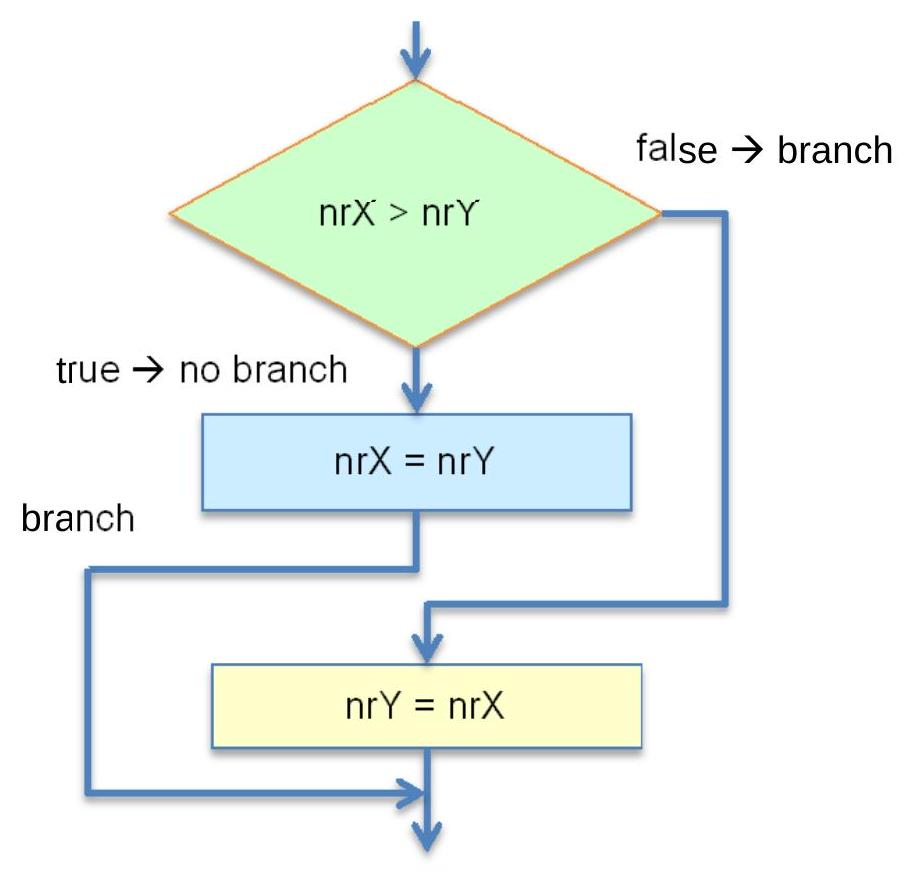
\includegraphics[width=\linewidth]{images/2025_01_02_7eee2d56b23c0199f878g-5}\\
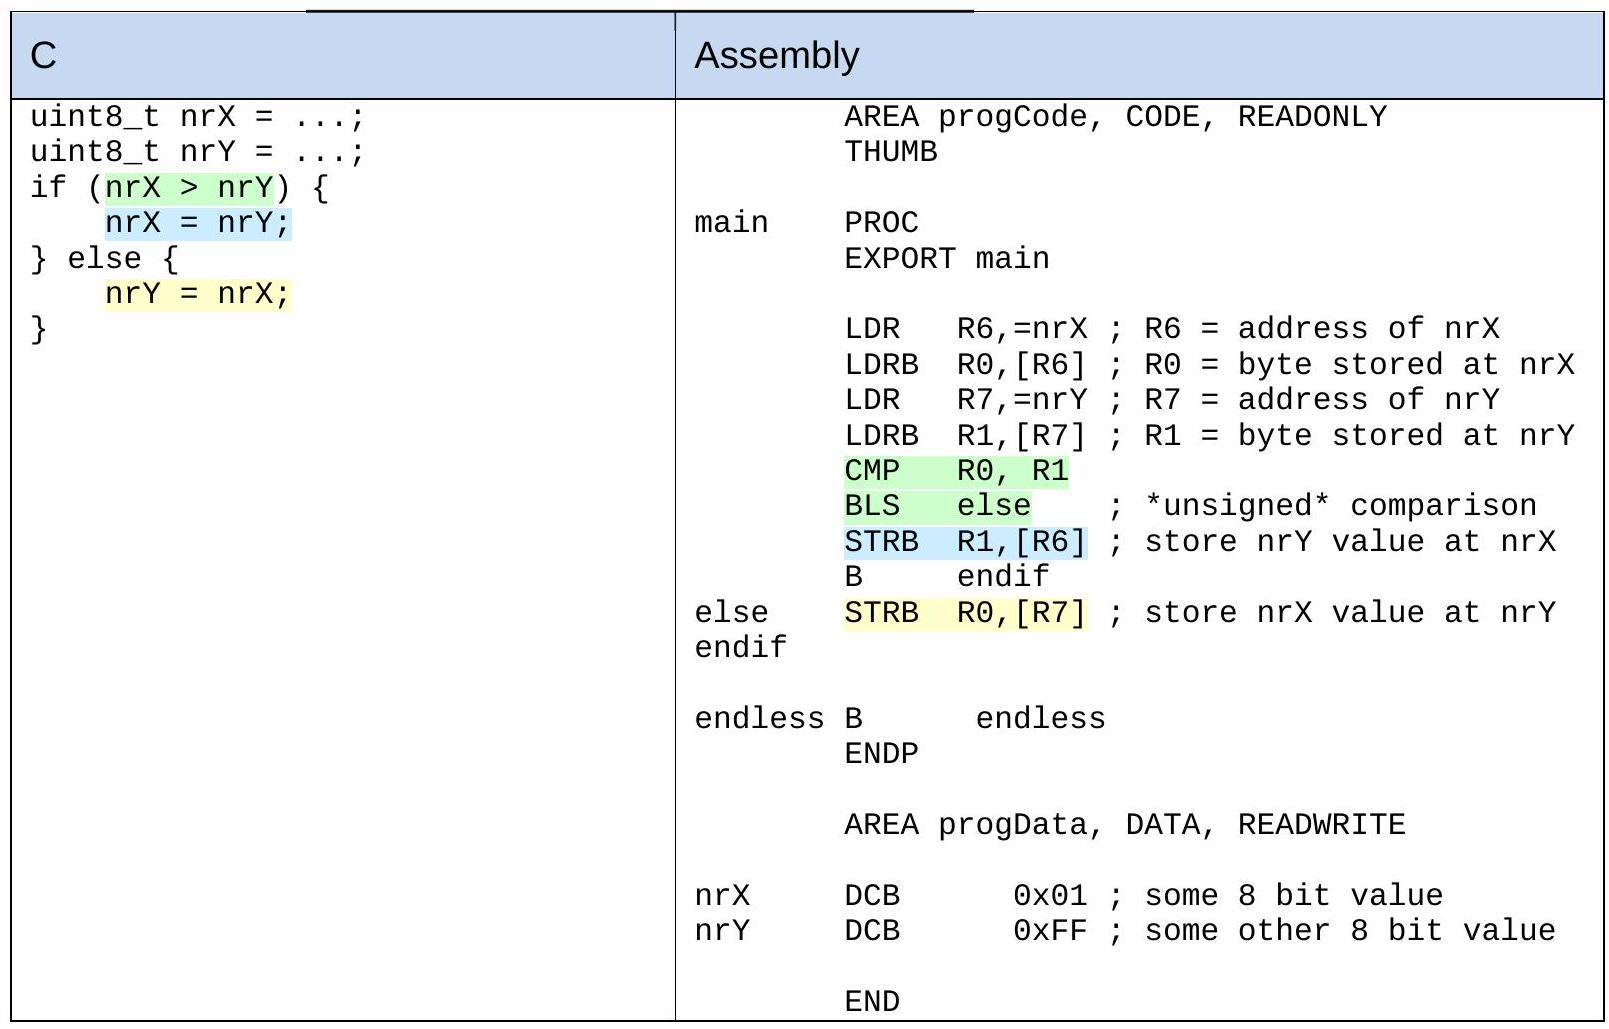
\includegraphics[width=\linewidth]{images/2025_01_02_7eee2d56b23c0199f878g-5(1)}\\
B) If-Then-Else with signed 8-bit variables\\
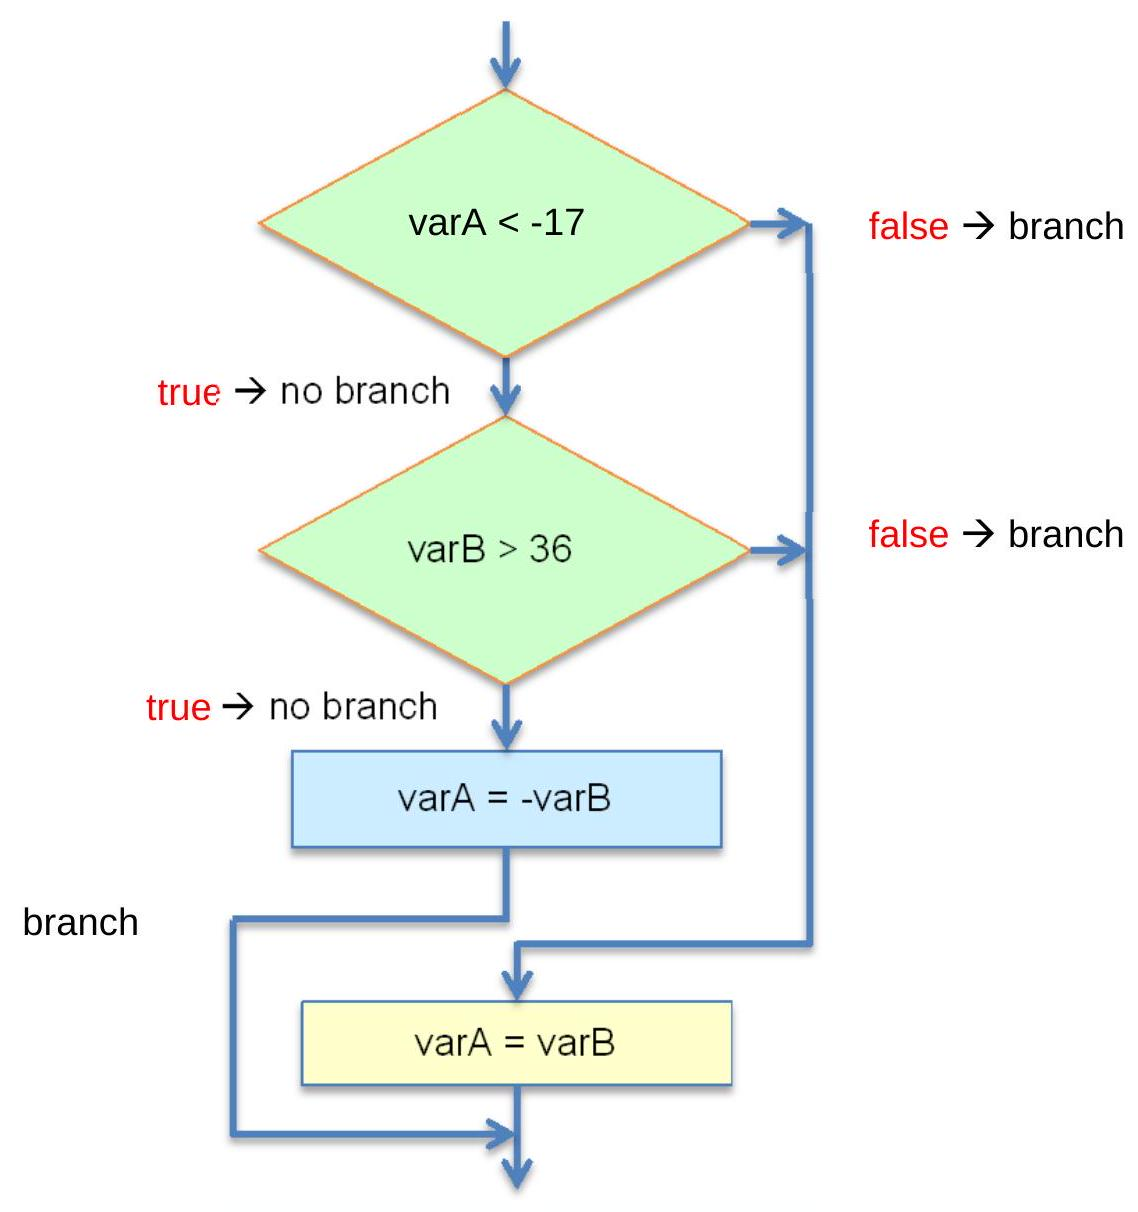
\includegraphics[width=\linewidth]{images/2025_01_02_7eee2d56b23c0199f878g-6}\\
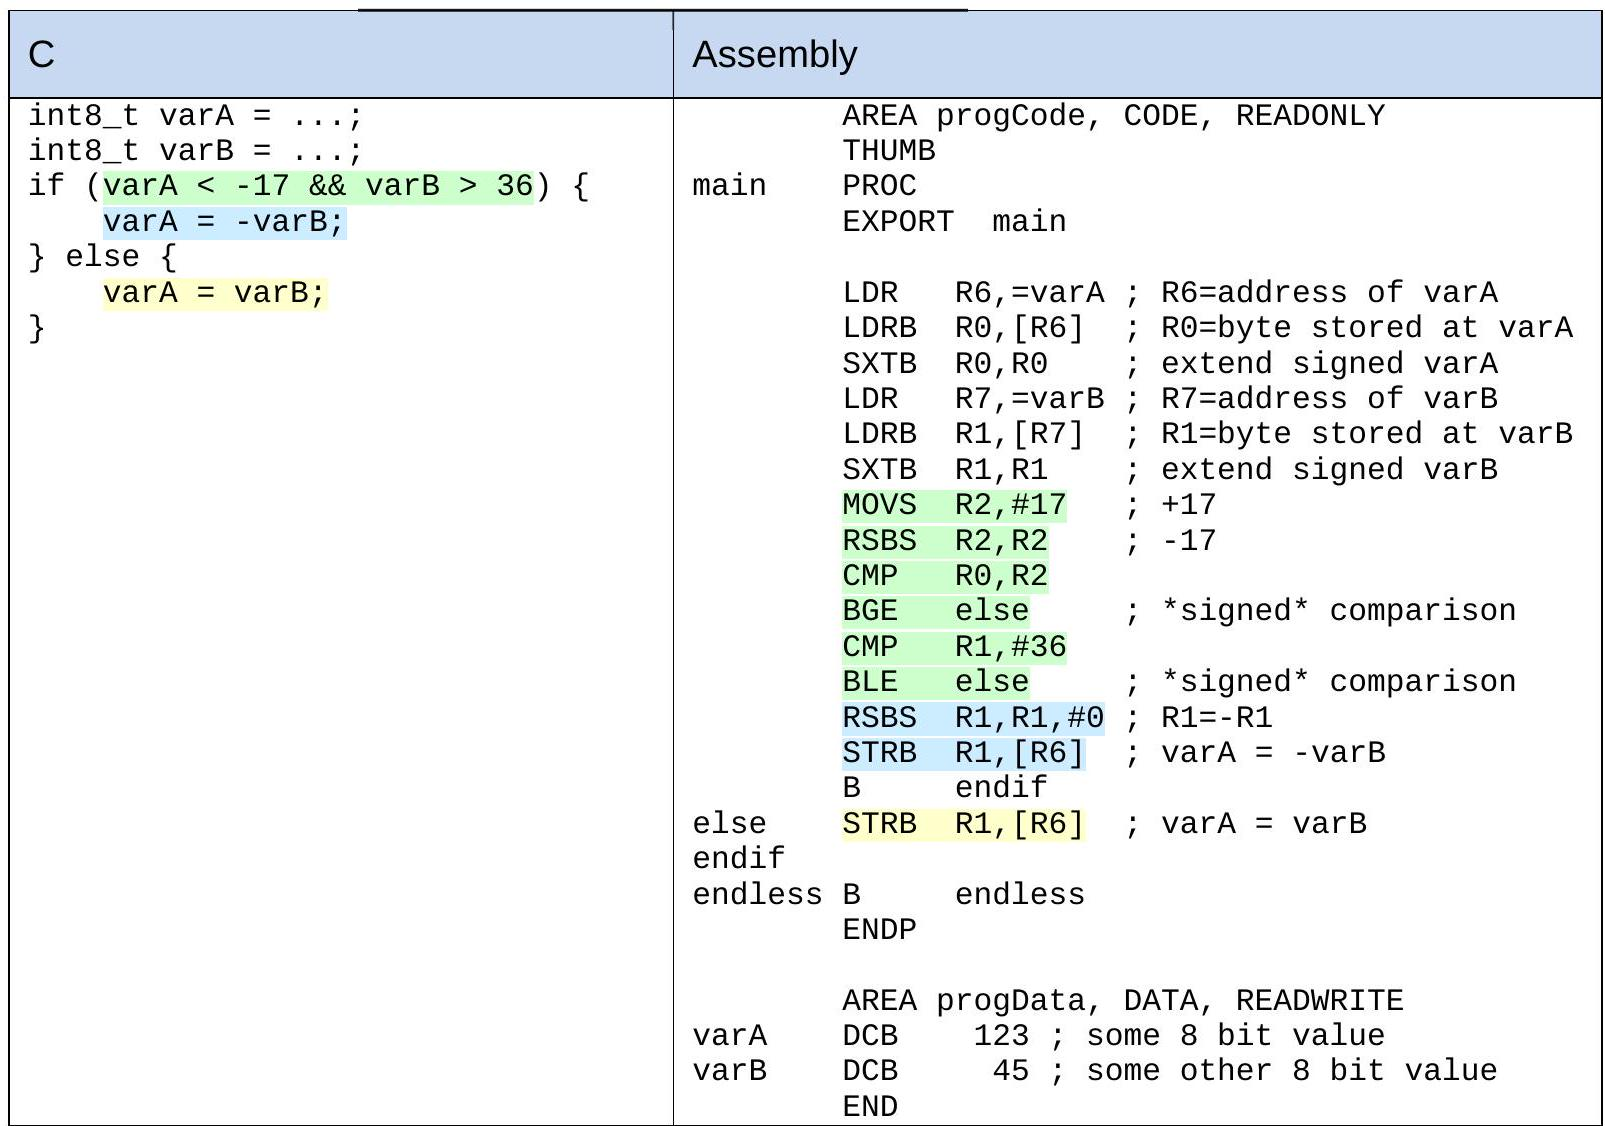
\includegraphics[width=\linewidth]{images/2025_01_02_7eee2d56b23c0199f878g-6(1)}\\
C) If-Then-Else with signed 16-bit variables\\
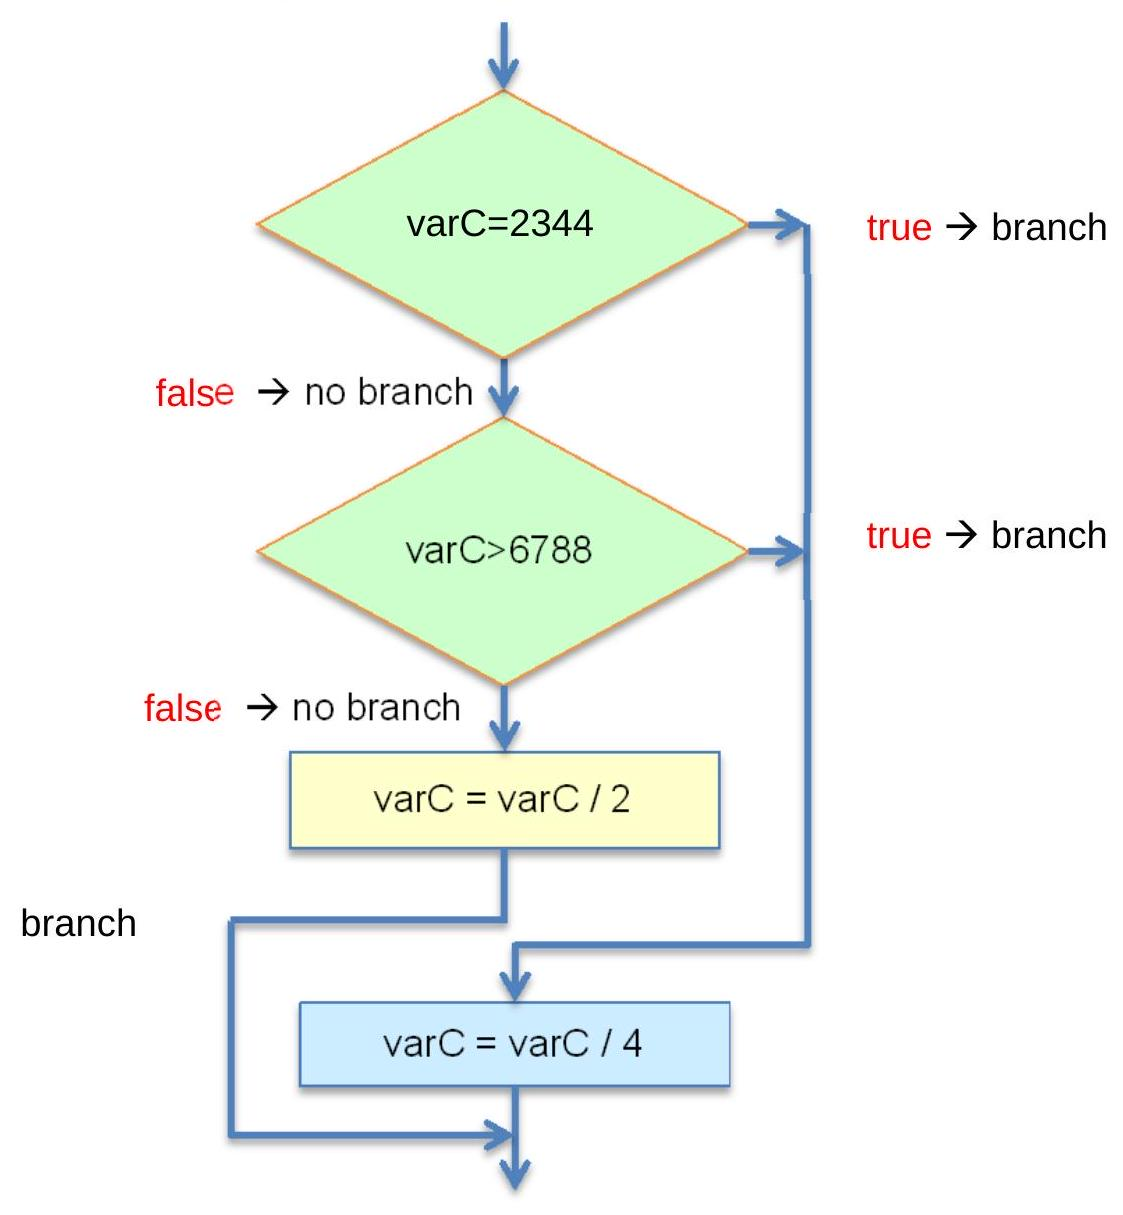
\includegraphics[width=\linewidth]{images/2025_01_02_7eee2d56b23c0199f878g-7(1)}

\begin{center}
\begin{tabular}{|c|c|}
\hline
C & Assembly \\
\hline
\texttt{int16\_t varC = ...; if (varC == 2344 || varC > 6788)\{ varC = varC / 4; \} else \{ varC = varC / 2; \}} & 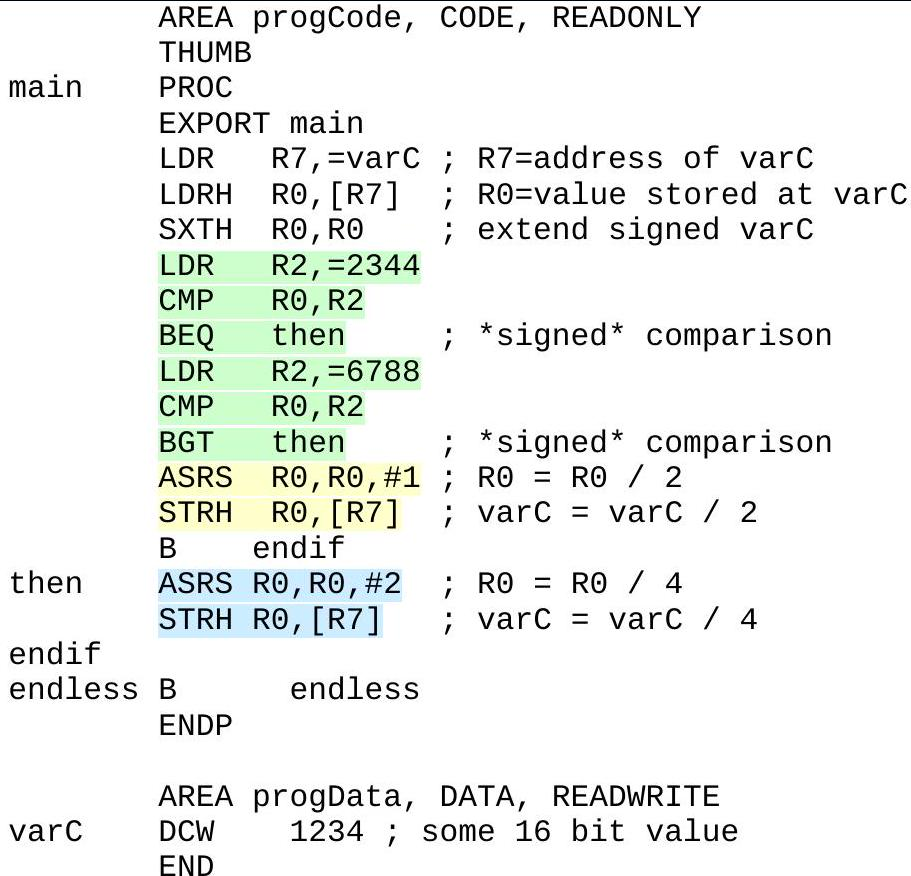
\includegraphics[width=\linewidth]{images/2025_01_02_7eee2d56b23c0199f878g-7}
 \\
\hline
\end{tabular}
\end{center}

\section*{Exercise 2:}
A) For-loop

\begin{center}
\begin{tabular}{|c|c|}
\hline
C & Assembly \\
\hline
\texttt{\#include <utils\_ctboard.h> \#include <stdint.h> ... int32\_t = 0; int32\_t count = 0; for(i = 0; i < 10; i++) \{ count++; \}} & 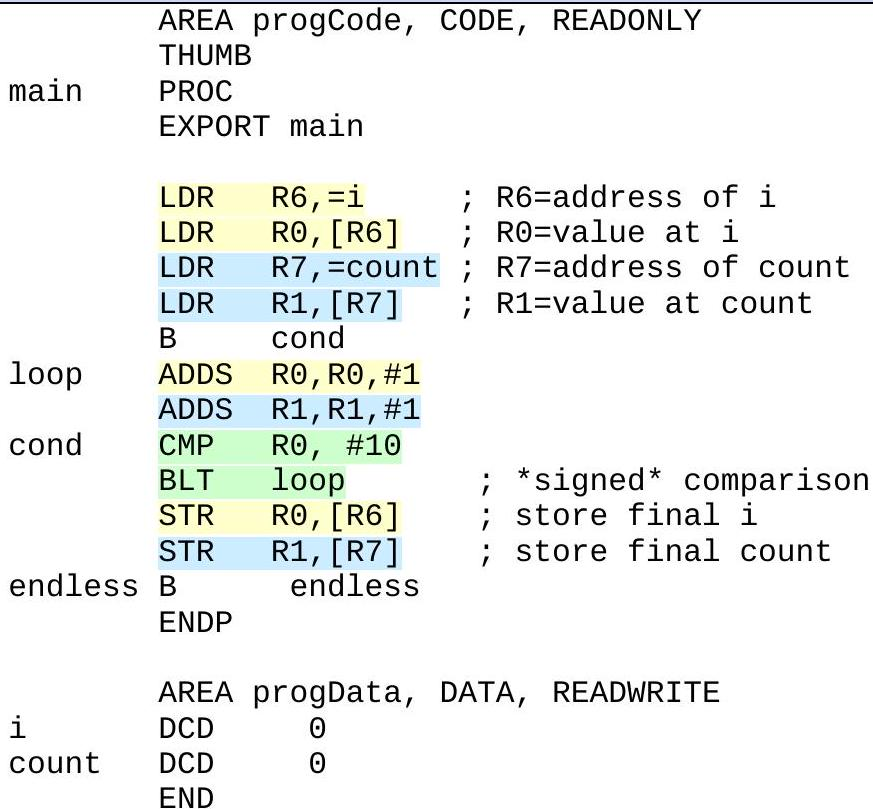
\includegraphics[width=\linewidth]{images/2025_01_02_7eee2d56b23c0199f878g-8}
 \\
\hline
\end{tabular}
\end{center}

B) Compare hand-crafted Assembly version to generated Assembly version\\
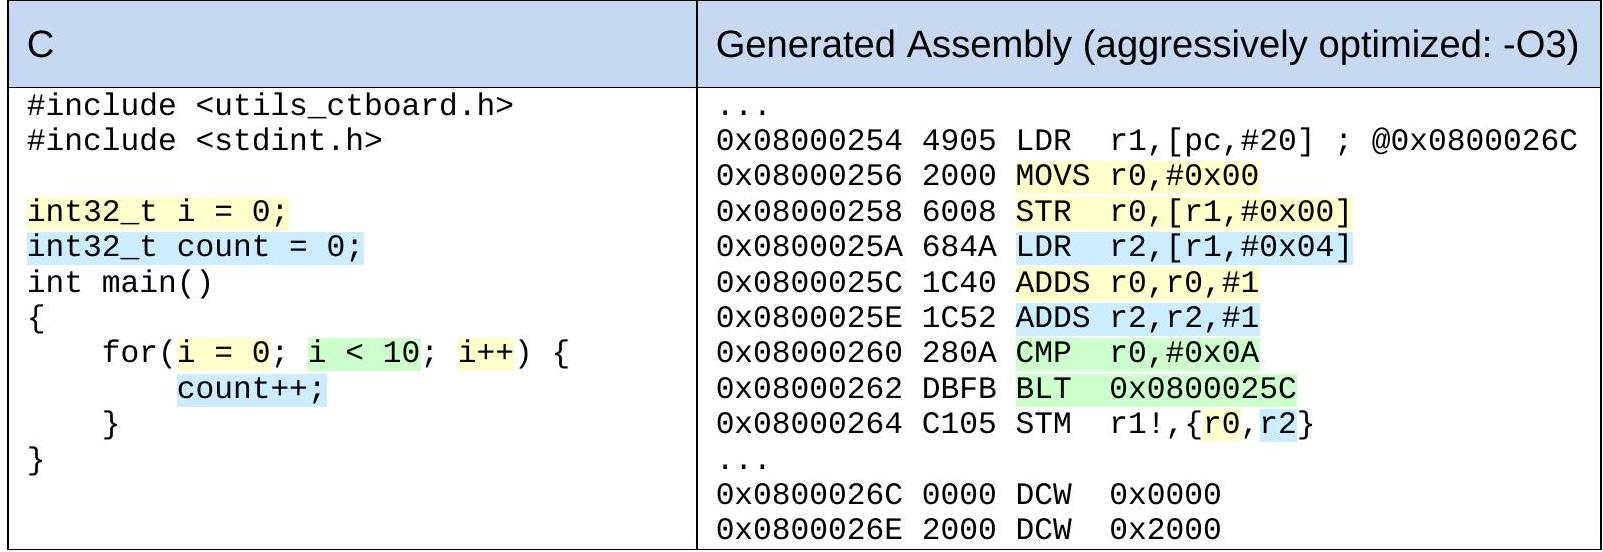
\includegraphics[width=\linewidth]{images/2025_01_02_7eee2d56b23c0199f878g-8(1)}

\section*{Exercise 3:}
A) The structorgram is

\begin{center}
\begin{tabular}{|c|c|}
\hline
\multicolumn{2}{|r|}{$\mathrm{R} 2=0$} \\
\hline
\multicolumn{2}{|l|}{while (R3 = srcstr[R2]) ! $=0$} \\
\hline
\multicolumn{2}{|l|}{\begin{tabular}{l}
\( \text { if (R3 >= } 60 \text { AND R3 <= 90) } \) \\
then else \\
\end{tabular}} \\
\hline
$\mathrm{R} 3=\mathrm{R} 3+32$ &  \\
\hline
\multicolumn{2}{|r|}{outstr[R2] = R3} \\
\hline
\multicolumn{2}{|r|}{INC R2} \\
\hline
\multicolumn{2}{|r|}{outstr[R2] = R3} \\
\hline
\end{tabular}
\end{center}

B) The resulting text is a null terminated string of all caps from the original string: THIS IS MY TESTSTRING